\section{Scheibe}
    \subsection{Definition}
        \begin{wrapfigure}[7]{r}{0.5\linewidth}
            \vspace{-3mm}
            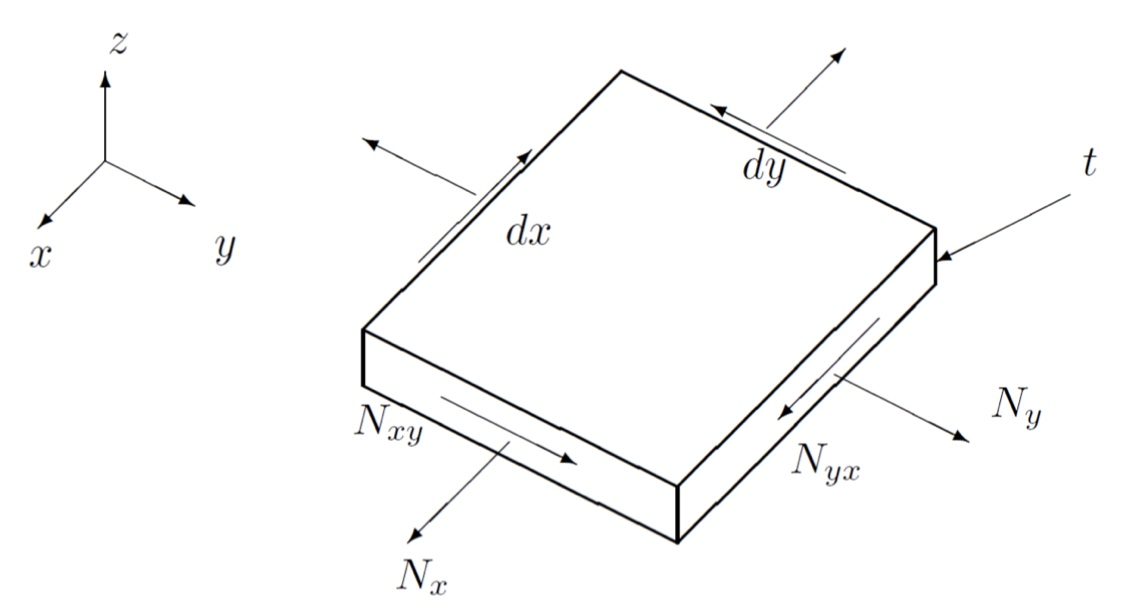
\includegraphics[width=\linewidth]{03/Scheibe}
        \end{wrapfigure}
        \textbf{Scheibenelement:} Dünnwandige Struktur mit Belastung in der Ebene. Äussere Kräfte dargestellt durch $N_x,N_y,N_{xy},N_{yx}$: Kräfte pro Längeneinheit ($\rightarrow$ Spannungen $\sigma_{xx},\sigma_{yy},\tau_{xy}$ über Dicke t integriert).

    \subsection{Annahmen}
        \begin{enumerate}[noitemsep]
            \item \textbf{Ebener Spannungszustand} ($\sigma_{zz},\tau_{xz},\tau_{yz}=0$)
            \item Übrige Spannungskomponenten sind konstant verteilt in z-Richtung (homogene Spannungsverteilung)
            \item Keine Volumenkräfte
            \item \textbf{Spannungsansatz} (GGB erfüllt)
        \end{enumerate}
        1, 2: Vernünftig, weil planare Dimensionen $\gg$ t \& keine Biegung. GGB reduziert sich zu: $\displaystyle\sigma_{xx,x} + \tau_{xy,y}=0$; $\sigma_{yy,y} + \tau_{xy,x}=0$
        $\rightarrow$Definiere $F(x,y)$ (Airy'sche Spannungsfkt) mit:\\ $\sigma_{xx}=F_{,yy}$; $\sigma_{yy}=F_{,xx}$; $\tau_{xy}=-F_{,xy}$.
        \\Aus Kompatibilitätsbedingung: $\varepsilon_{xx,yy}+\varepsilon_{yy,xx}=2\varepsilon_{xy,xy}$ \\$\rightarrow F_{,xxxx}+F_{,yyyy}+2F_{xxyy}=0 \Leftrightarrow\Delta\Delta F=0$.
        \\Funktion $F(x,y)$ so wählen, damit RB erfüllt.
	\\Da statischer Ansatz $\rightarrow$ Minimierung der komplementären Deformationsenergie.
    \subsection{Scheibe mit Loch}
        \begin{center}
            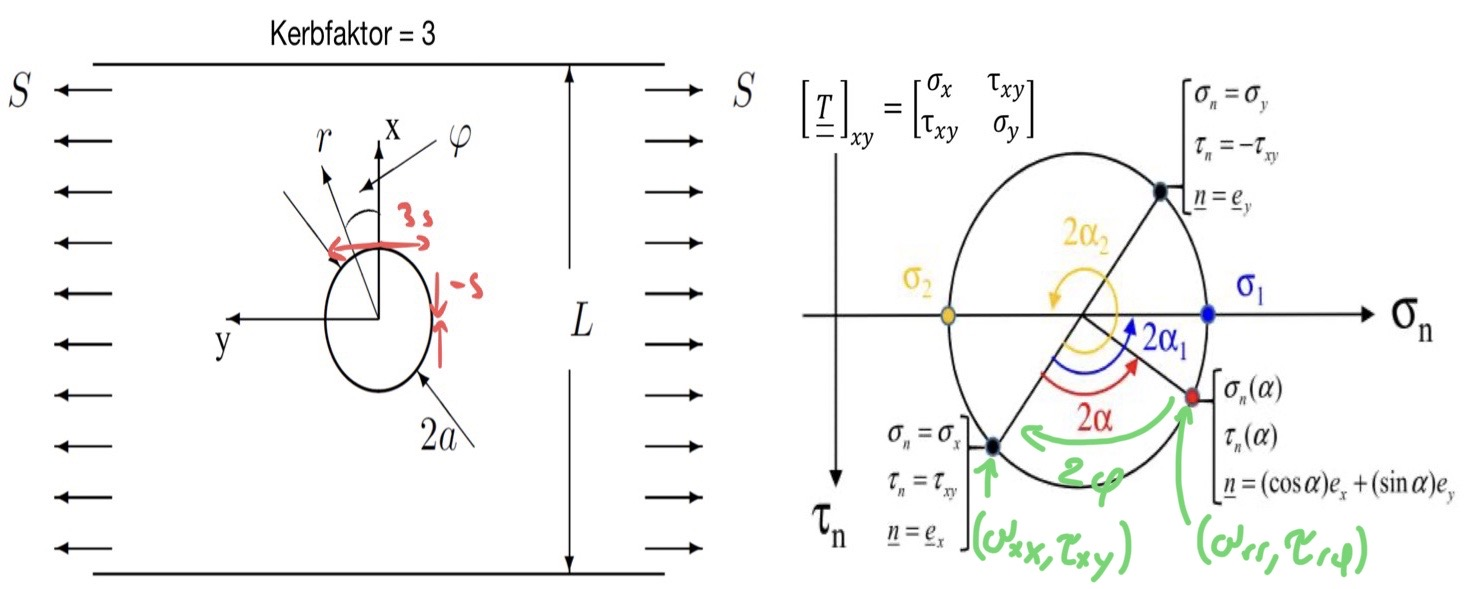
\includegraphics[width=0.9\linewidth, height=30mm]{03/mohr_and_loch_2.JPG}
            $\tiny{\lambda_{1,2}= \frac{1}{2}(\sigma_x+\sigma_y)\pm\sqrt{\frac{1}{4}(\sigma_x-\sigma_y)^2+\tau_{xy}^2}}$\\
            $\sigma_{\overset{\textcolor{blue}{rr}}{\textcolor{red}{\varphi\varphi}}}=\sigma_{xx}\overset{\textcolor{blue}{cos^2(\alpha)}}{\textcolor{red}{sin^2(\alpha)}}+\sigma_{yy}\overset{\textcolor{blue}{sin^2(\alpha)}}{\textcolor{red}{cos^2(\alpha)}} \cpm 2\tau_{xy}sin(\alpha)cos(\alpha)$\\
            $\tau_{r\varphi}=(\sigma_{yy}-\sigma_{xx})sin(\alpha)cos(\alpha)+\tau_{xy}(cos^2(\alpha)-sin^2(\alpha)$
        \end{center}
\columnbreak
        \begin{itemize}
            \item Lochradius a $\ll$ L
            \item Belastung durch uniforme, einachsige Spannung S in grosser Entfernung vom Loch
            \item Spannungsfreie Rissflanken ($r = a; \forall\varphi\in\mathbb{R} $): $\sigma_{rr}=0, \tau_{r\varphi}=0$
        \end{itemize}
        \textbf{Superposition} von mehreren Spannungen \& Spannungsrichtungen möglich.Schubspannungen in Hauptspannungen umwandlen.
        \begin{center}
            $\sigma_{\overset{\textcolor{blue}{\varphi\varphi}}{\textcolor{red}{rr}}}=\frac{s}{2}\left(1\cpm\frac{a^2}{r^2}\cpm cos(2\varphi)\left(1+3\frac{a^4}{r^4}\textcolor{red}{-4\frac{a^2}{r^2}}\right)\right)$
            $\tau_{r\varphi}=\frac{s}{2}\left(1-3\frac{a^4}{r^4}+2\frac{a^2}{r^2}\right)sin(2\varphi)$
        \end{center}

    \subsection{Scheibe mit Riss}
        Spannungsfreie Rissflanken ($\forall r, \varphi=\pm\pi$): $\sigma_{\varphi\varphi}=0, \tau_{r\varphi}=0$
        \begin{center}
            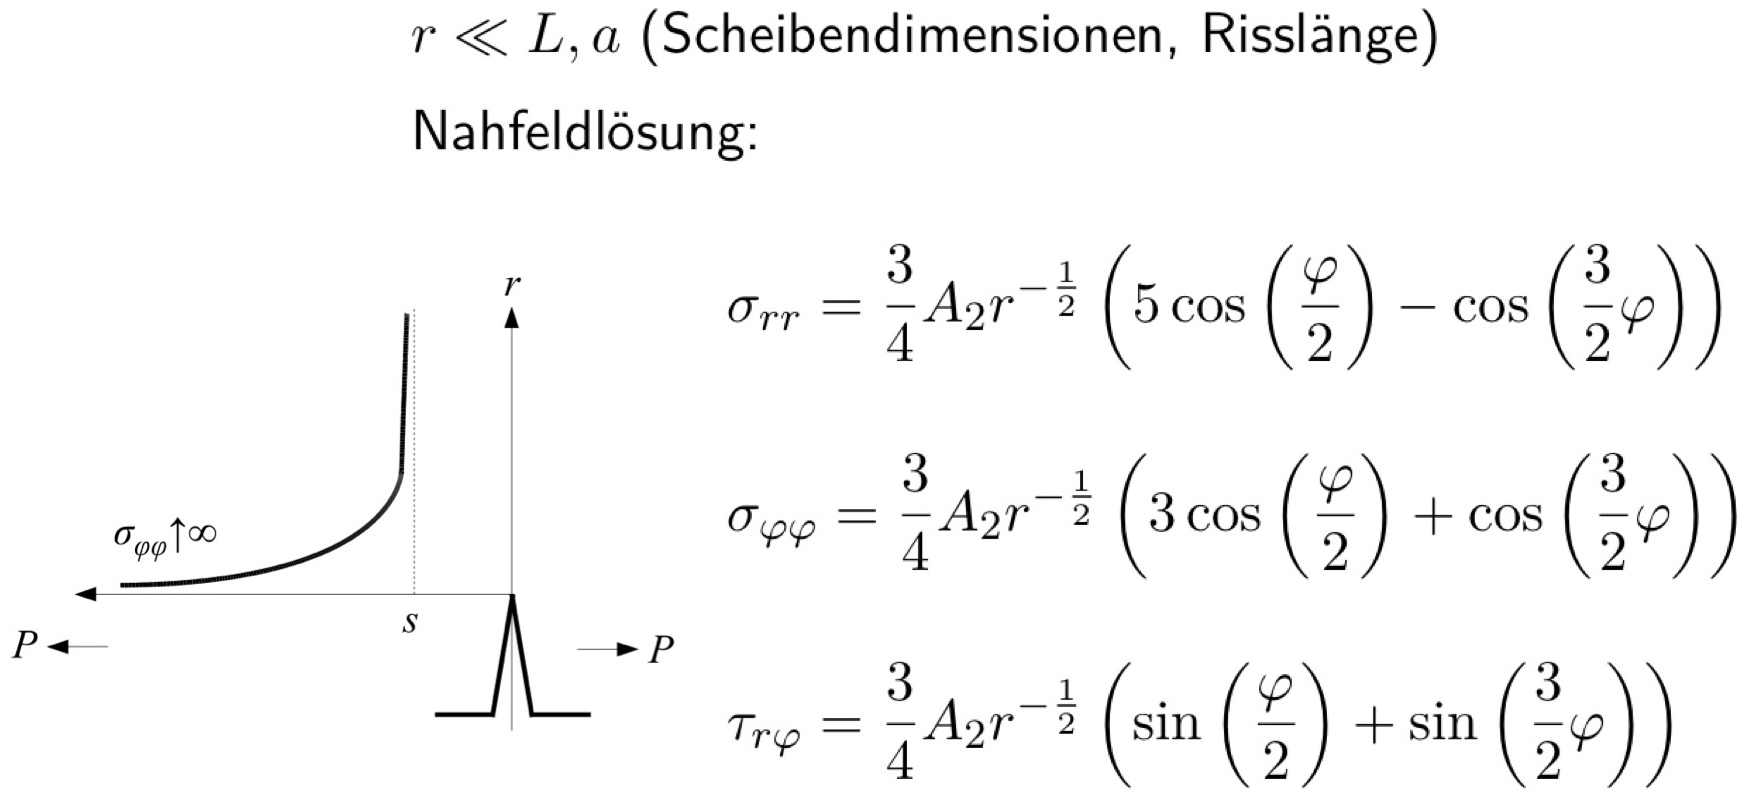
\includegraphics[width=70mm, ]{03/Scheiberiss}
        \end{center}
\vspace{-2mm}
